%%% template.tex
%%%
%%% This LaTeX source document can be used as the basis for your technical
%%% paper or abstract.

%%% The parameter to the ``documentclass'' command is very important.
%%% - use ``review'' for content submitted for review.
%%% - use ``preprint'' for accepted content you are making available.
%%% - use ``tog'' for technical papers accepted to the TOG journal and
%%%   for presentation at the SIGGRAPH or SIGGRAPH Asia conference.
%%% - use ``conference'' for final content accepted to a sponsored event
%%%   (hint: If you don't know, you should use ``conference.'') 

\documentclass[conference]{acmsiggraph}

\usepackage[utf8]{inputenc}  
\usepackage[T1]{fontenc}  

%%% Make the ``BibTeX'' word pretty...

\def\BibTeX{{\rm B\kern-.05em{\sc i\kern-.025em b}\kern-.08em
    T\kern-.1667em\lower.7ex\hbox{E}\kern-.125emX}}

\title{Real Time NeuroEvolution of Augmenting Topologies in video games}

%%% TODO: Mettre les adresses de l'école
\author{Guillaume Ambrois\thanks{e-mail:guillaume.ambrois@gmail.com}, Sébastien Gaulier\thanks{e-mail:sebastien.gaulier@gmail.com}\\ESGI, Paris}
\pdfauthor{Guillaume Ambrois & Sébastien Gaulier}

%%% TODO: Ajouter des mots clés
\keywords{video game, artificial intelligence, machine learning, NeuroEvolution of Augmenting Topologies}

\begin{document}

%%% This is the ``teaser'' command, which puts an figure, centered, below 
%%% the title and author information, and above the body of the content.

%%% TODO: Changer l'image
 \teaser{
   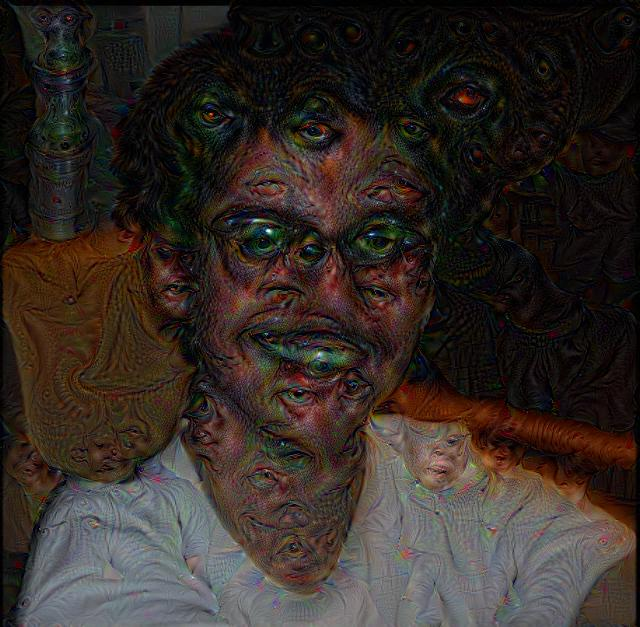
\includegraphics[height=1.5in]{images/sampleteaser}
   \caption{NERO, showcase video game for rtNEAT}
 }

\maketitle

\begin{abstract}

In this poster, we will talk about how we can achieve real time NEAT, using rtNEAT, an open source and free to use library originally written by Kenneth Stanley from the University of Texas.

\end{abstract}

\keywordlist

%% Required for all content. 

\copyrightspace

\section{Introduction}

Artificial Intelligence is one of the fields that advances the most in video games, but there is still a tremendous work to be done. AI is still only scripted behaviors : we tell the agent what to do depending on the situation.

NeuroEvolution of Augmenting Topologies (NEAT) allows us to weight parameters and structures of networks, so we can tune our agents' AI by rewarding them for a good behavior (like shooting an enemy) and punishing them for a bad behavior (like taking cover from enemy shots).

\section{Using rtNEAT}

We use the UE4 as an engine to build our game. rtNEAT comes as source files, so we just had to include one header and we were able to start using the library.

Lorem ipsum dolor sit amet, consectetur adipiscing elit. Curabitur gravida arcu sit amet mi molestie, et aliquet augue hendrerit. Curabitur eget luctus risus. Nulla gravida, leo eget porttitor ullamcorper, elit augue finibus mi, eu mollis nunc eros id mi. Pellentesque vel blandit ligula. Etiam augue leo, mattis eu ultricies sed, tempor vitae mauris. Etiam sit amet lectus scelerisque, vehicula ipsum ac, scelerisque tellus. Cras sit amet faucibus nulla. Vestibulum et dolor non felis tristique condimentum. Morbi non erat at ex viverra faucibus. Proin sed dapibus mi. Ut interdum mi sit amet lobortis congue. Nulla nibh massa, sollicitudin nec sodales in, viverra nec risus. Pellentesque habitant morbi tristique senectus et netus et malesuada fames ac turpis egestas. Nullam pretium, magna nec iaculis convallis, nulla ante viverra mi, sed tristique eros tortor quis magna. Nunc ut purus sit amet neque elementum consectetur.

\section{Our approach}

Lorem ipsum dolor sit amet, consectetur adipiscing elit. Curabitur gravida arcu sit amet mi molestie, et aliquet augue hendrerit. Curabitur eget luctus risus. Nulla gravida, leo eget porttitor ullamcorper, elit augue finibus mi, eu mollis nunc eros id mi. Pellentesque vel blandit ligula. Etiam augue leo, mattis eu ultricies sed, tempor vitae mauris. Etiam sit amet lectus scelerisque, vehicula ipsum ac, scelerisque tellus. Cras sit amet faucibus nulla. Vestibulum et dolor non felis tristique condimentum. Morbi non erat at ex viverra faucibus. Proin sed dapibus mi. Ut interdum mi sit amet lobortis congue. Nulla nibh massa, sollicitudin nec sodales in, viverra nec risus. Pellentesque habitant morbi tristique senectus et netus et malesuada fames ac turpis egestas. Nullam pretium, magna nec iaculis convallis, nulla ante viverra mi, sed tristique eros tortor quis magna. Nunc ut purus sit amet neque elementum consectetur.Lorem ipsum dolor sit amet, consectetur adipiscing elit. Curabitur gravida arcu sit amet mi molestie, et aliquet augue hendrerit. Curabitur eget luctus risus. Nulla gravida, leo eget porttitor ullamcorper, elit augue finibus mi, eu mollis nunc eros id mi.

\bibliographystyle{acmsiggraph}
\nocite{*}
\bibliography{template}
\end{document}
